
\section{Introduction}
	\IEEEPARstart{T}{he} aim of this project was to investigate how the diversity of an genetic algorithm's population effects the performance of Multi-Layer Perception Neural Network trained by said algorithm. 
	A substantial amount of research has already been conducted into how the effectiveness of Hyper-heuristic's can be improved by encouraging diversity in the individual sub-heuristics. This investigation was designed to assess if a similar approach to hyper-heuristic diversity could be applied to an genetic algorithm to improve it's fitness.
	
\section{Approach}
	Investigation was conducted by exploring how different types of Parent Selection, Child Crossover, Mutation, and Immigrant Injection can alter the overall diversity of a genetic algorithm's population and how in turn that effects the overall fitness of the algorithm.
	
	\subsection{Background}
		Previous research has shown evidence that increasing the diversity of the individual heuristics in  a hyper-heuristic can improve the overall fitness of said hyper-heuristic\cite{Hong16112004} \cite{hart2017constructing}. This effect is caused by the way sub-heuristics of similar fitness will tend to operate upon data in a similar manner, inversely sub-heuristics with a greater difference in fitness will tend operate upon data in a vastly different behaviour. By creating a hyper-heuristic out of a number of randomly chosen sub-heuristics, the hyper-heuristic has a better chance of avoiding reaching a local maxima, as opposed to a hyper-heuristic comprising of a number of elite sub-heuristics which may reach a local optima significantly faster.
		
		This projects aims to investigate if a similar approach can be taken in regards to genetic algorithms, by comparing operators that produce various levels of diversity in within the population of the algorithm.
	
	\subsection{Algorithm Design}
		A simple genetic algorithm of similar style to supplied version was used throughout this investigation. Unless otherwise stated, a single generation of the algorithm was as follows:

		\begin{algorithm}[H]
			\caption{Genetic Algorithm Pseudocode}
			A random population is generated\\
			Two individuals are selected from the population as parents\\
			Two children are generated from  the parents\\
			The children are mutated\\
			Children replace two worst individuals in the population
		\end{algorithm}
		
		Upon completion, the fittest chromosome produced by the algorithm were used as the weights for a multi-layer perception neural network, which attempted to perform a function estimation using pre-supplied training data. Once that algorithm was run for a predetermined number of generations, a final test using a separate set of data was used to determine the overall effectiveness of the neural network, and in thus, the effectiveness of the genetic algorithm. Details of selection, crossover and mutation methods are presented below.  
			
	\subsection{Algorithm Operators}
	
	\begin{figure*}[]
		\centering
		\subfloat[Single point crossover]{
			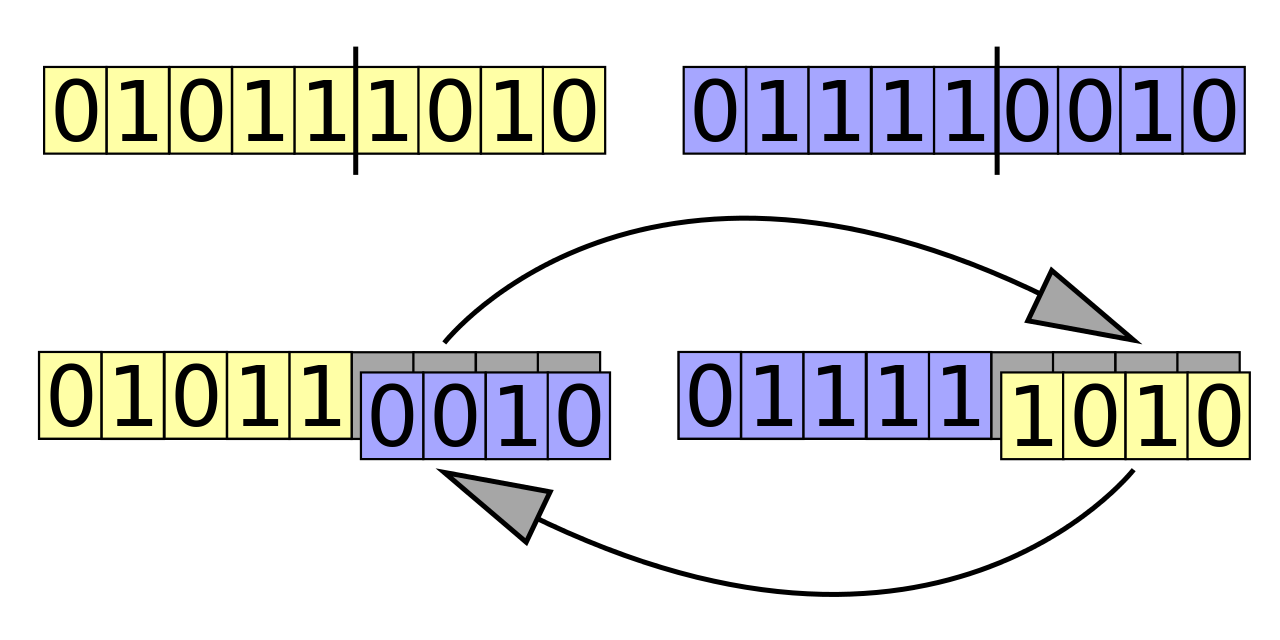
\includegraphics[width=2.5in]{crossover_single}%
			\label{fig_cross_single}
		}
		\hfil
		\subfloat[Double point crossover]{
			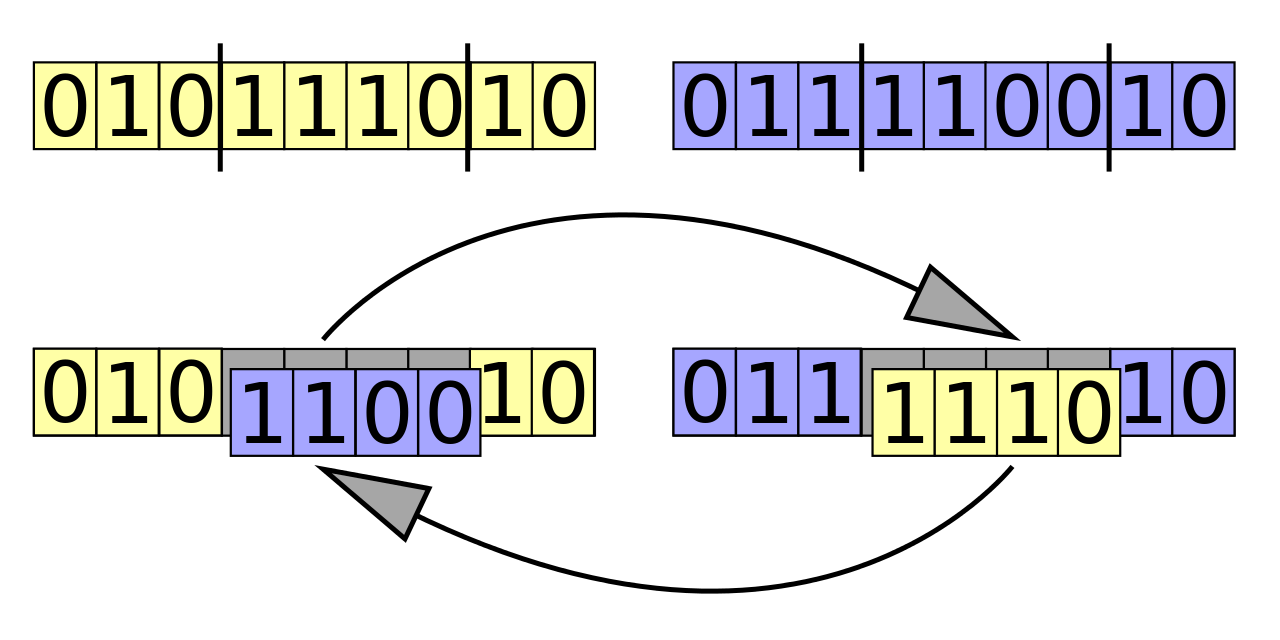
\includegraphics[width=2.5in]{crossover_double}%
			\label{fig_cross_double}
		}
		\newline
		\subfloat[Uniform crossover]{
			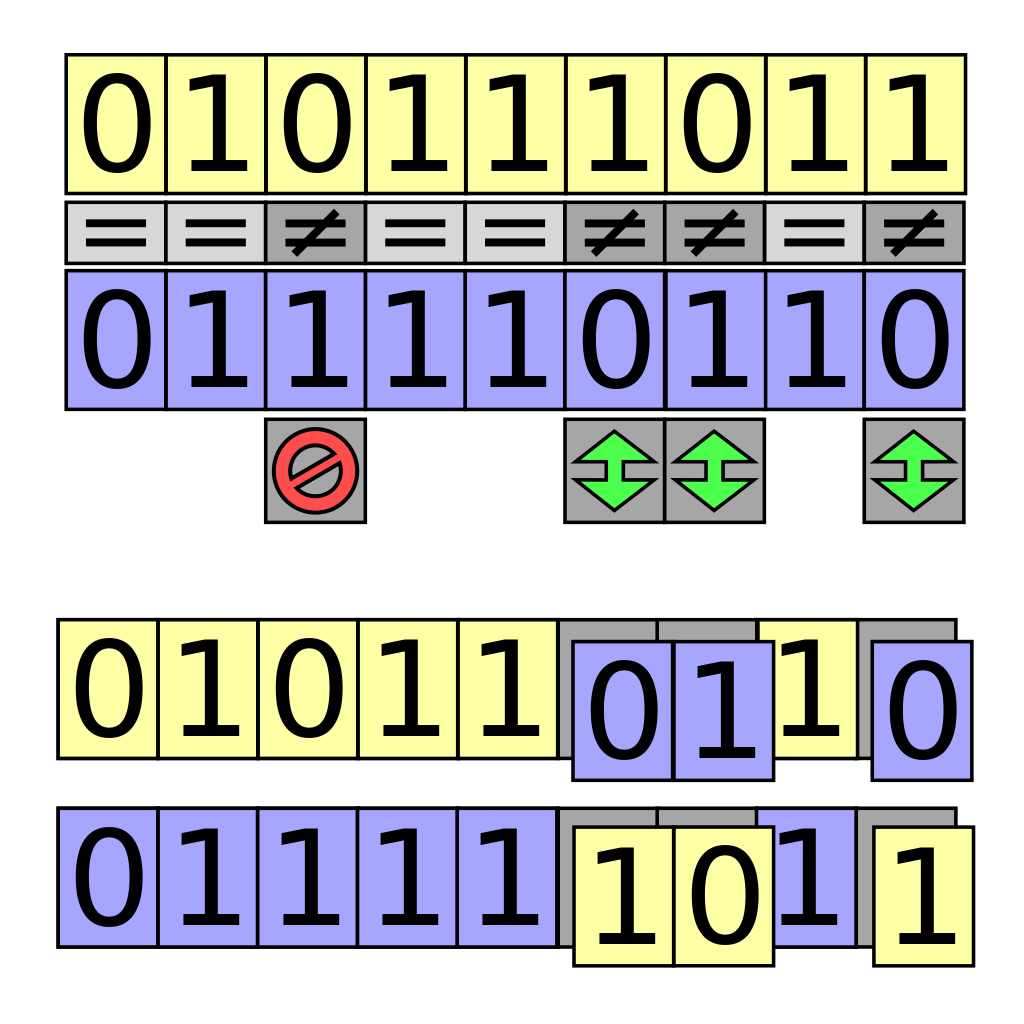
\includegraphics[width=1.25
			in]{crossover_uniform}%
			\label{fig_cross_uni}
		}
		\caption{Three examples of crossover function.}
		\label{fig_cross}
	\end{figure*}
	
		\subsubsection{Selection}
			While the provided \texttt{selectRandom} function was a perfectly valid solution to increasing the diversity of selected parents, alternative selection functions had to be designed to allow for comparison.
			
			\texttt{selectRandom}: The provided selection method operates by simply choosing two random individuals from the population. This selection function should be considered the most diverse, as every individual in the population has an equal chance of being selected to become a parent, regardless of their fitness
	
			\texttt{selectElite}: This selection method operates by choosing the two individuals with the best and second-best fitness. From a ignorant approach, this may seem to be a valid section tactic, in reality however this method is likely to cause the population to reach a local maxima within a relatively small number of generations. \texttt{selectElite} was included in this investigation to provide evidence that a lack of diversity in the population may be deferential to its potential fitness.
			
			\texttt{selectTournament}: This function was designed to randomly choose a designated number of individuals and the individual in the group with the best fitness goes forward as a parent. The number of individuals in the tournament directly alters the selection pressure, lager tournaments have a smaller chance of a weaker individual being chosen for crossover. This selection method should prove adequate in diversifying the population, however it is unlikely to be as pronounced as the \texttt{selectRandom} function.
			
			\texttt{selectRoulette}: A roulette selection has the potential to pick any individual in the population, proportional to its fitness  While individuals with high fitness are more likely to be selected by this function, it is not guaranteed, ensuring this function is suitable for the diversification of the population.
		
		\subsubsection{Crossover}
			All  crossover methods utilised in this project produced a pair children which were then introduced to the algorithm population by replacing the two individuals with the worst fitness. Crossover is the most typical way to add diversity to an genetic algorithm, however the children's similarity to their parents is determined by the type of crossover used.			
	
			\texttt{crossoverClone}: The provided crossover function produces a pair of children, each identical to one of the parents. The use of this kind crossover will result in the eventual homogenization of the algorithm's population - significantly reducing the diversity of the chromosomes. 
		
			\texttt{crossoverSingle}: A single-point crossover method uses a random number to determine a crossover point in two newly created children chromosomes. Each child is then given a number of genes from one parent, until reaching the crossover point when they then receive genes from the other parent. This crossover method produces two inversely mirrored children. In extreme cases can produce two children identical to the parents, reducing the overall diversity of the population by introducing duplicates. 
			
			\texttt{crossoverDouble}: Extremely similar to the  \texttt{crossoverSingle} function, with the caveat being that two crossover points are generated. With the addition of a second pivot point on which to swap which parent is passing genes, the chances of producing children similar to the parents is reduced, assuming that the two parents are not already similar in terms of genes.
			
			\texttt{crossoverUniform}: Unlike the previous segment based crossovers, a uniform crossover function operates on a gene level. Each gene in a child is copied from one of the two parents depending on the value of a randomly generated number e.g. On the value of 0 the first parent's gene is used, on the value of 1 the second parent's gene is copied. Like the other crossover functions, \texttt{crossoverUniform} produces a set of mirrored children. This crossover method has the potential to produce the most diverse children from a set of parents. 
			
		\subsubsection{Mutation}
			Mutation of chromosomes is yet another area of a genetic algorithm where diversity can be introduced. No form of mutation was provided, so a simple boundary mutation function was designed within the algorithm presented. Mutation was only applied to child chromosomes produced by a cross over function.
			
			\texttt{mutateBoundary}: This mutation function operates over every gene in a chromosome, producing a random \texttt{double} between 0 and 1 for each one. If the double is less than a predetermined value (\texttt{mutateRate}) then the current gene is altered by adding  or subtracting a second predetermined value (\texttt{mutateChange}) to the gene. Once all the genes in a chromosome gave been considered for mutation, any genes that were pushed outside their maximum or minimum boundary are then brought back in line.
		
	\subsection{Neural Network}
		As the primary goal of this report was to investigate how the diversity of the genetic algorithm's population changed its effectiveness, very few of the Neural network's parameters were changed or investigated.
		
		\texttt{geneMax} \& \texttt{geneMin}: The values of 5.0 and -5.0 were used respectively for the maxim and minimum possible values of gene for each chromosome. While the systematic altering and testing of these values could have led to a superior solution. Leaving them at the default values ensured the other test could be compared fairly.
		
		\texttt{hiddenNodes}: The number of nodes in the hidden layer was the second tunable parameter of the neural network. Once again, it was opted to leave this parameter at a predetermined value for all tests, in this case 5, for a number of reasons. Firstly, this investigation was more focused on the tuning of the genetic algorithm rather than the neural network and secondly, in order to produce an optimal result the parameter would potential have to be readjusted every time another variable was, leading to a enormous number of tests needing to be run.
		
		%The number of nodes in the hidden layer was the one neural network parameter that was changed from the default. Preliminary testing indicated that when approximating functions A and B 5 hidden nodes produced the best result. When approximating function C however, 2 hidden nodes proved to be the most effective. These values were used in all future tests to ensure consistent and fair comparison. 
		
\section{Methodology}
	\subsection{Experiment Parameters}
		To ensure fair comparison, and to comply with the project specification, the following parameters were used for all tests, unless otherwise stated:
		\begin{itemize}
			\item Each algorithm was run for a maximum 10000 generations.
			\item The average final fitness of 50 iterations was used to determine the effectiveness of algorithm.
			\item Each iteration used a different seed to prevent chances of identical executions.
		\end{itemize}
	
	\subsection{Experiments}
		With the generic parameters outlined, the following experiments were conducted:
		\begin{itemize}
			\item The effect of population size on overall fitness.
			\item The effect of different selection methods on overall fitness.
			\item The effect of different crossover methods on overall fitness.
		\end{itemize}
	
		All experiments were conducted on each of the functions using the same parameters. During the execution of experiments the parameters used and the best fitness of each generation were logged to a \texttt{.csv} file for ease of access and later analysis.

\section{Results}
	\subsection{Population Experiment}
		This test was chosen to be conducted first, as the information it  would reveal would be beneficial in selecting the population size of future tests. The experiment was executed as follows:
		
		The test was run 50 times, starting at a population of 10 and increasing by 10 for each subsequent iteration i.e. the first test had a population of 10 and the final test had a population of 500. The \texttt{selesctRandom} and \texttt{crossoverSingle} algorithm features were chosen for this test, in an attempt to reduce the chances of local maxima.
		
		As can be seen from Figures \ref{chart_pop_a}, \ref{chart_pop_b},  and \ref{chart_pop_c} as the population of each algorithm increases so to does the fitness improve. This is as we would expect, the larger population size, the more diverse the initial population reducing the algorithm's chances from reaching a local maxima. 
		
		\begin{figure}[h]
			\centering
			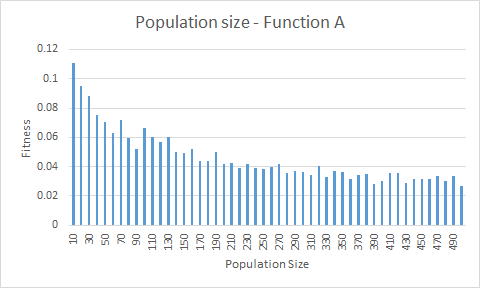
\includegraphics[width = 0.5\textwidth]{pop_a}
			\caption{A chart indicating the correlation between population and fitness for Function A.}
			\label{chart_pop_a}
		\end{figure} 

		\begin{figure}[h]
			\centering
			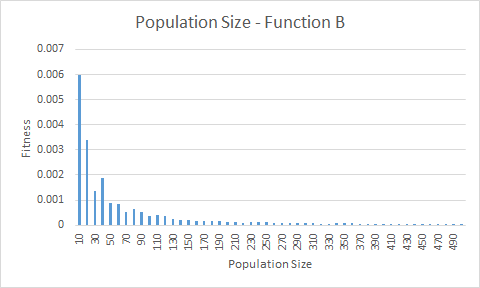
\includegraphics[width = 0.5\textwidth]{pop_b}
			\caption{A chart indicating the correlation between population and fitness for Function B.}
			\label{chart_pop_b}
		\end{figure}

		\begin{figure}[h]
			\centering
			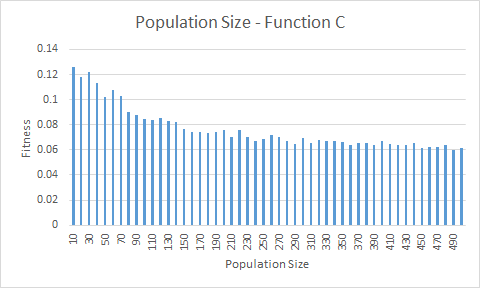
\includegraphics[width = 0.5\textwidth]{pop_c}
			\caption{A chart indicating the correlation between population and fitness for Function C.}
			\label{chart_pop_c}
		\end{figure}
	
	After the completion of these initial tests, a population size of 500 was utilised for all future experiments, as at that size the benefit of adding more individuals was reaching a diminishing return as well as increasing the time needed to execute the algorithm.

	\subsection{Low Diversity Experiment}
		Once the initial population experiment was complete, testing proper could take place. The Low Diversity Experiment was designed as a control, using the \texttt{selectElite} and \texttt{crossoverClone} functions with the aim of producing a population of low diversity. The results of said test are visible in Table \ref{tab_low}.
		
		\begin{table}[h]
			\centering
			\caption{Low Diversity Experiment}
			\label{tab_low}
			\begin{tabular}{|c|c|c|}
				\hline
				\textbf{Function A} & \textbf{Function B} & \textbf{Function C} \\ \hline
				0.02813             & 0.00005             & 0.06280             \\ \hline
			\end{tabular}
		\end{table}
	
		While the results of this experiment reveal very little on their own, they do provide a benchmark  from which other methods can be compared. It should be noted that while the algorithms in this test will have produced a homogenized population, they may not have produced a poor fitness due to the nature of genetic algorithms. 
		
		\subsection{Random Selection Experiment}
			With a control value now determined the assessment of the various selection and crossover techniques could continue, starting with \texttt{selectRandom} selection function.
			
			The algorithms were each tested using the \texttt{crossoverSingle}, \texttt{crossoverSingle}, \texttt{crossoverDouble}, and \texttt{crossoverUniform} crossover methods, and the results are visible in Table \ref{tab_rand}.
						
			\begin{table}[h]
				\centering
				\caption{Random Selection Experiment Results}
				\label{tab_rand}
				\begin{tabular}{|c|c|c|c|}
					\hline
					\textbf{}           & \textbf{Single} & \textbf{Double} & \textbf{Uniform} \\ \hline
					\textbf{Function A} & 0.02710         & 0.02894         & 0.03535          \\ \hline
					\textbf{Function B} & 0.00004         & 0.00005         & 0.00005          \\ \hline
					\textbf{Function C} & 0.07208         & 0.06344         & 0.06447          \\ \hline
				\end{tabular}
			\end{table}
		
		The results of this experiment are mixed, while Functions A and B were able to produce results superior to the Low Diversity Experiment, there was not a clear improvement in performance when utilising the more diversifying crossover methods. The cause for these results may be due to a number of reasons. One hypothesis is that the \texttt{selectRandom} function  was unable to select suitably fit parents for crossover. A solution could be created by increasing the selection pressure of the algorithm, potential improving the fitness by selecting fitter parents. 
									
		\subsection{Roulette Selection Experiment}
			The \texttt{selectRoullete} method can be viewed as a midway between elite and random selection, there is the potential for any individual in the population to be selected for crossover but a bias for the selection of fitter members exists.
			
			\begin{table}[h]
				\centering
				\caption{Roulette Selection Results}
				\label{tab_rou}
				\begin{tabular}{|c|c|c|c|}
					\hline
					& \textbf{Single} & \textbf{Double} & \textbf{Uniform} \\ \hline
					\textbf{Function A} & 0.03463         & 0.03245         & 0.02897          \\ \hline
					\textbf{Function B} & 0.00006         & 0.00005         & 0.00004          \\ \hline
					\textbf{Function C} & 0.07539         & 0.07267         & 0.07127          \\ \hline
				\end{tabular}
			\end{table}
		
			The results of this experiment show a clear trend  in the overall improvement of fitness when more diversifying crossover methods are utilised. For each function tested the \texttt{crossoversingle} produced a worse fitness than \texttt{crossoverDouble}, which in turn was worse than \texttt{crossoverUniform}. This is as hypothesised in the initial designing of the project. This result seems to indicate that when the parents are chosen randomly with some form of selection pressure, a more diverse population will improve the fitness. It should be noted  that none of the results produced were superior to those of Low Diversity or Random Selection Experiments. 
			
\section{Conclusion}
	While this project was unable to prove that a more divers population would produce a lower fitness, some interesting results were found. When the results of Roulette Selections Experiment are considered by themselves, the proposed hypothesis appears true but when the results are compared against  those of other less diverse algorithms it becomes clear that there is no benefit to diversification of the population, at least for the problems tested in this project. 

\section{Future Work}
	The original intent of this project was to complete a thorough investigation of both the genetic algorithm and the neural network, including the altering and analysis of parameters not reviewed in this paper or recommended as apart of the specification. Initial work was undertaken, but it was revealed that an error in the fitness analysis had resulted in the production of incorrect values, leading to false positives and assumptions without data to back them up. With all the previously collected data and analysis invalidated, data  had to be recollected and processed, not leaving ample time to complete all the desired tests.
	
	Future work would consist of a full analysis of all the parameters relating to the algorithm and the neural network, with the aim of producing more definitive evidence either for or against the diversification of a genetic algorithm's population.